\chapter{\acl{hrc} System}
\label{chapter:hrc_system}

This chapter reviews the hardware and software tools used during development and the software developed to support a practical implementation of action anticipation in human-robot collaboration. In particular, \autoref{section:system_architecture} details the system architecture including the available hardware and the software tools chosen to establish communication between all the parts. \autoref{section:methodologies} describes the research methodologies employed in this dissertation. Section \autoref{section:first_experiments} delves into the implementation of initial experiments which integrate all the parts to simulate anticipatory behavior. \autoref{section:materials_methods_final_remarks} provides final remarks about the content of this chapter and its connection to the next.

\section{System Architecture}
\label{section:system_architecture}

The work described in this dissertation is part of the AUGMANITY project\footnote{AUGMANITY website: \url{https://www.augmanity.pt}} that aims to develop technologies to support people operating in industrial environments. The experimental setup comprises the integration of both hardware and software components in a prototype collaborative cell (LARCC) at the Laboratory for Automation and Robotics (LAR) located in the Department of Mechanical Engineering at the University of Aveiro, as illustrated in \autoref{fig:LARCC}. The LARCC is equipped with a UR10e collaborative robot and multimodal sensor devices, including three LiDAR Velodyne sensors and four Orbbec 3D cameras distributed throughout the work volume. The software architecture is built upon the \acf{ros} middleware \cite{Quigley2009}, providing a robust framework for communication and coordination among the various components. In this context, this section provides a description of the materials used during this study and the methodological approaches followed to face the key challenges. 

\begin{figure}[ht]
    \centering
    \includegraphics[width=0.75\columnwidth]{figs/LARCC_prototype.pdf}
    \caption{Prototype collaborative cell LARCC}
    \label{fig:LARCC}
\end{figure}

\if{0}
\begin{figure}[!ht]
\centerline{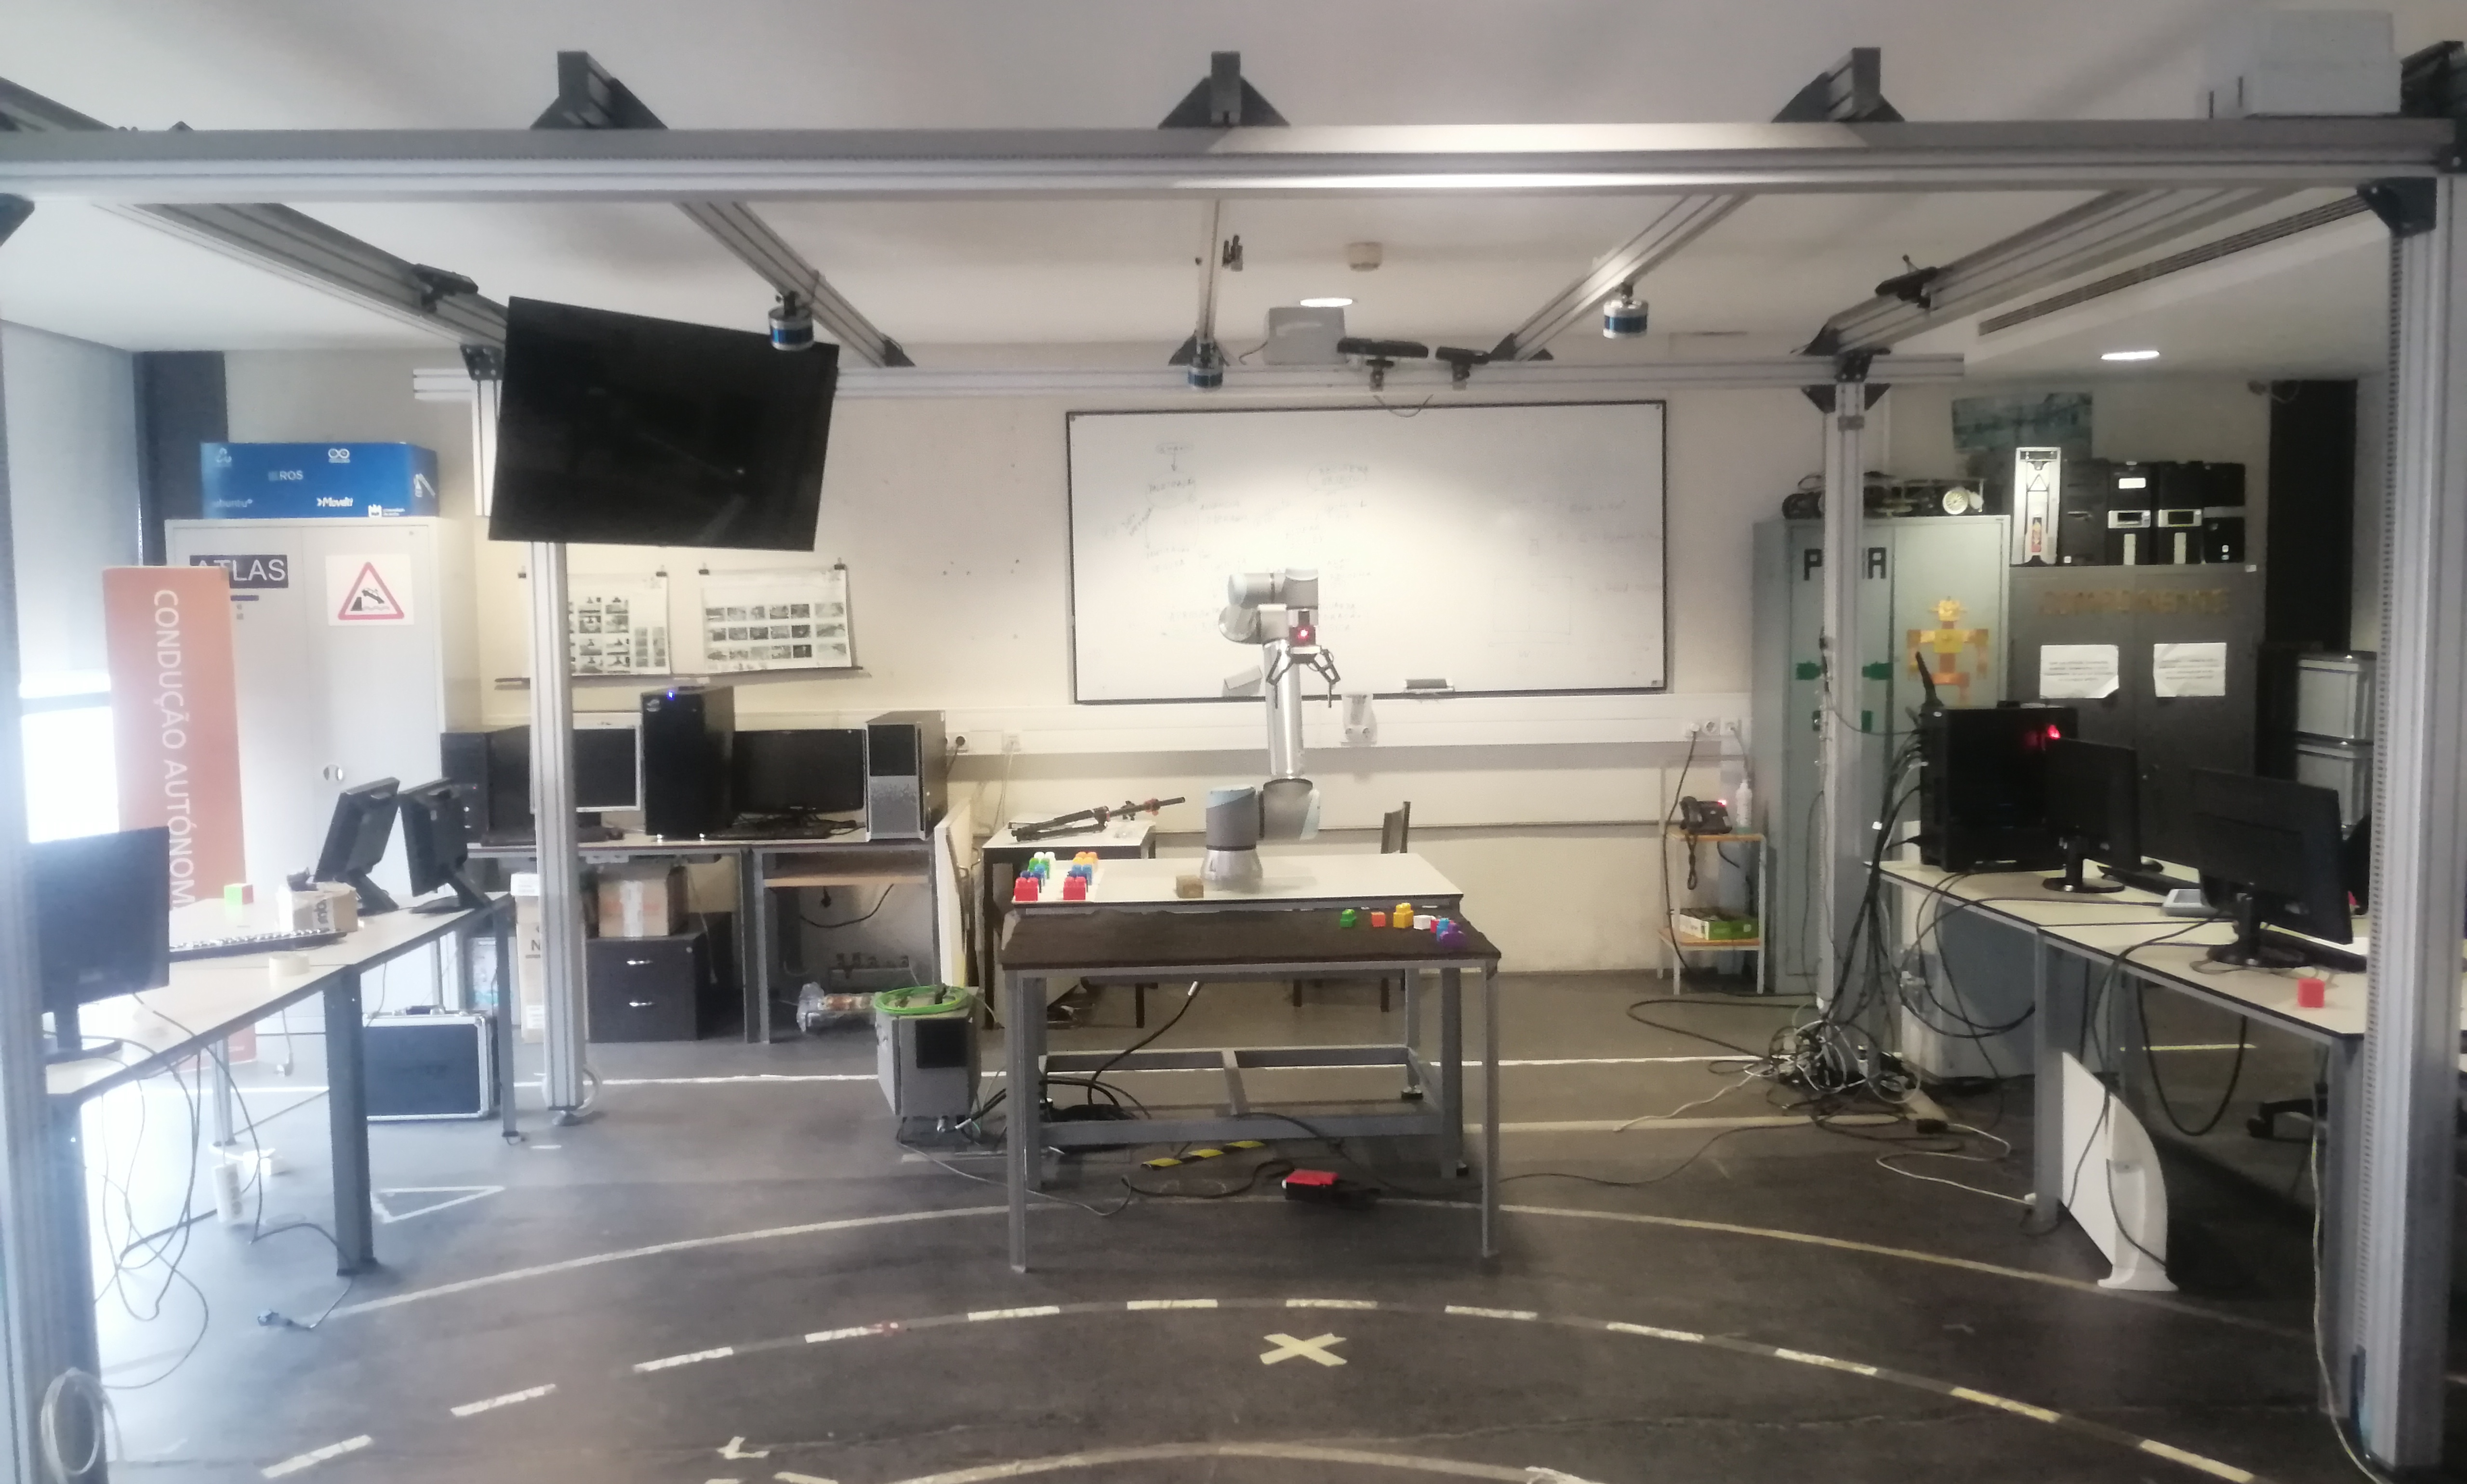
\includegraphics[width=0.9\textwidth, trim={0 5cm 0 0}, clip]{figs/setup2.jpg}}
\caption[setup]{LAR hardware setup}
\label{fig:LARCC}
\end{figure}
\fi

\subsection{\acf{ros}}

\acs{ros}\cite{ROS2}\footnote{\acs{ros} 1 documentation: \url{https://wiki.ros.org}}\footnote{\acs{ros} 2 documentation: \url{https://docs.ros.org/en/humble}} is an open-source collection of tools and software libraries used to develop a robotics application and, in this work, it is used to establish communication throughout all of the infrastructure. \acs{ros} was chosen due to the hardware abstraction it offers given that it contains driver packages to deal with some hardware devices, allowing for easier communication with the robot and the cameras. Other relevant features include:
\begin{itemize}
    \item \textbf{message broker}: every process in the project is a node in the \acs{ros} network and communicates with the other nodes mainly through topics (asynchronous publish/subscribe streaming of data) or services (synchronous RPC-style communication).
    \item \textbf{code reuse}: executables and packages are written to be as independent as possible, making the developer able to reuse them in another project.
    \item \textbf{rich ecosystem}: there are several open-source packages available to the developer that can be easily integrated.
    \item \textbf{scalability}: given that the nodes are so loosely coupled, it allows for node distribution.
    \item \textbf{language independence}: nodes can be written in any language since communication is established through well-defined objects.
    \item \textbf{data visualization}: there are tools to visualize the data and the functioning of the system in real-time, such as Rviz.
    \item \textbf{simulator support}: \acs{ros} has support for simulators with Gazebo being the most common.
\end{itemize}

For this system, the \acs{ros} 1 Noetic distribution was chosen over the more recent \acs{ros} 2 distributions so as to take advantage of work already done by other members of the AUGMANITY project at the University of Aveiro.

\subsection{Perception System}
\label{subsection:perception_system}

In order to capture the necessary information from the environment, two Orbbec Astra Pro RGBD cameras were used. This camera model was developed by Orbbec Technologies and it is frequently used in computer vision and robotics \cite{AstraPro}. Among the available cameras, it was chosen since it allowed to capture both color and depth images.

\begin{figure}[ht]
\centerline{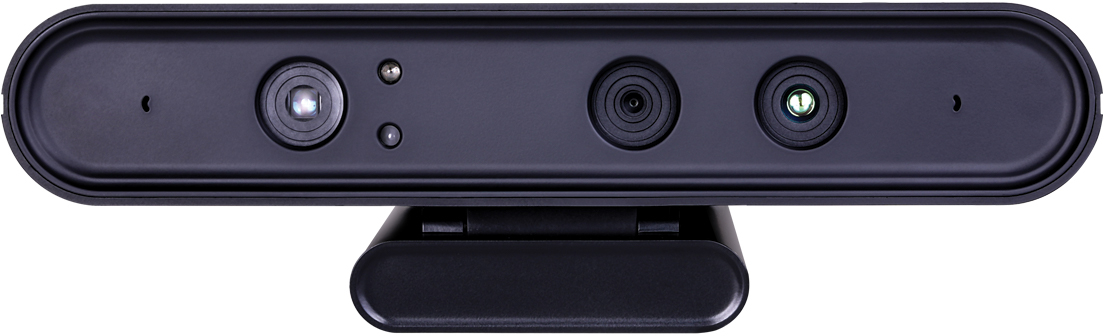
\includegraphics[width=0.6\textwidth]{figs/AstraPro.jpg}}
\caption[Orbbec Astra Pro]{Orbbec Astra Pro \cite{AstraPro}}
\label{fig:orbbec_astra_pro}
\end{figure}

In the experimental setup, one of the cameras is placed above the workspace facing downwards allowing the perception of the objects in the table through the color image and the position of the user through the depth image. The second camera is above and slightly behind the robot to capture the user in front of the robot with the images from this camera being the ones used in the keypoint detection models. The communication with the cameras is established through ROS with the $usb\_cam$ package being used for the color image and the $ros\_astra\_camera$ package being used for the depth image. In order to have better control over the lightness in the environment, only artificial lighting was used and the back-light compensation was raised to the maximum in the $usb\_cam$ configurations. Then the frame rate was also set to 10 frames per second in both cameras given that none of the following image processing tasks require a high frame rate.

As said before, the color image of the first camera is used to detect objects in the environment. These objects are blocks of specific colors and therefore they can be identified with color segmentation, which is done with the help of OpenCV\footnote{OpenCV documentation: \url{https://docs.opencv.org/4.x/}}, a popular computer vision library. With this library, the image from the camera is initially cropped to a specific region of interest consisting of the table area, which is then converted from BGR to HSV given that the intervals of a color are more reliable in this representation. From the HSV image and the color intervals, a mask is obtained for each color. These masks are then subject to a closing morphological operation to reduce any possible noise. Finally, the resulting areas are considered an object if they surpass a certain area threshold further reducing noise.

On the other hand, the depth image is used to obtain the position of the human in the workspace by cropping it to a certain region of interest corresponding to where the user would normally be and then detecting the highest point.

\subsection{Manipulator Arm Control}
\label{subsection:manipulator_arm_control}

The collaborative robot available for this work is a UR10e model which was developed by Universal Robots. This model has six degrees of freedom with six rotational joints, allows for payloads up to \SI{12.5}{\kilogram}, and has a reach of \SI{1300}{\milli\metre} being suitable for tasks such as machine tending, palletizing, and packaging\cite{UR10e}. In this work, the robot is equipped with a 2F-140 gripper developed by Robotiq, commonly used together with robot models from Universal Robots\cite{robotiq_gripper}.

\begin{figure}[ht]
    \centerline{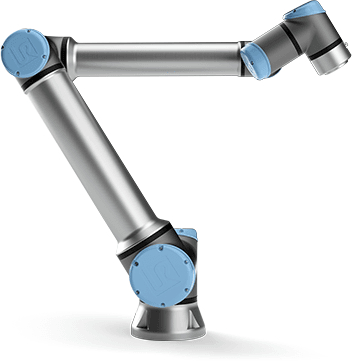
\includegraphics[width=0.4\textwidth]{figs/UR10e.jpg} \ \ 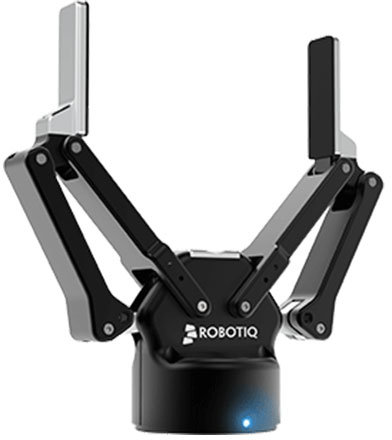
\includegraphics[width=0.35\textwidth]{figs/robotiq-2f-140.jpg}}
    \caption[UR10e Collaborative Robot and Robotiq 2F-140 Gripper]{UR10e Collaborative Robot \cite{UR10e_image} and Robotiq 2F-140 Gripper \cite{robotiq_gripper}}
    \label{fig:ur10e}
\end{figure}

Both the robot and the gripper have \acs{ros} packages containing their drivers making their integration easier. The planning and execution of the arm movements are done through the MoveIt\footnote{MoveIt documentation: \url{https://ros-planning.github.io/moveit_tutorials}} framework, which is a widely-used open-source framework for robotics applications involving motion planning, manipulation, 3D perception, kinematics, control, navigation, and collision checking, with \acs{ompl} being chosen to handle the motion planning tasks.

The configurations of the drivers and MoveIt was already done by other members of the AUGMANITY project and can be found on Github\footnote{Github LarCC Repository: \url{https://github.com/afonsocastro/larcc_interface}} along with a higher-level API that encloses that logic. During this work, an additional feature to stop movements was added.

\subsection{Computational Systems}

The tasks involved in this work, such as training deep-learning models and analyzing images in real-time require high computational resources. To handle the real-time processing of images and robot control, the central computer present in the setup was used. To handle the deep-learning model training, the deep-learning research server from LAR was used, codenamed Deeplar:
\begin{itemize}
    \item AMD RyzenTM Threadripper 2950X;
    \item Four NVIDIA GEFORCE® RTX 2080 Ti;
    \item 128GB DDR4 RAM.
\end{itemize}

The model training in Deeplar is executed using docker images, which allows multiple people to use the computer with each having their own isolated training environment with their own dependencies. The images used to design and train machine learning models in this work are based on the latest TensorFlow official image for GPUs.

TensorFlow is one of the most popular machine learning frameworks along with Pytorch. In this work, the former was chosen over the latter since the higher-level API allowed for faster development. The main features of Tensorflow\footnote{Tensorflow documentation: \url{https://www.tensorflow.org/api_docs}} are:
\begin{itemize}
    \item \textbf{prepare data}: load data, data pre-processing and data augmentation;
    \item \textbf{build models}: design and train custom models with little code or use pre-trained ones (transfer learning);
    \item \textbf{deploy models}: helps using models in different platforms such as locally, in the cloud, in a browser, or in mobile;
    \item \textbf{implement MLOps}: run models in production, tracking their performance and identifying issues.
\end{itemize}

\section{Methodologies/Research Methods}
\label{section:methodologies}

This section covers the methodologies employed in this dissertation to research anticipatory systems.

\subsection{Keypoints Detection Frameworks}
\label{subsection:keypointdetection}

This subsection reviews OpenPose, OpenPifPaf, and Mediapipe which are three projects containing models to detect keypoints in images, such as the human skeleton joints.

\subsubsection{OpenPose}

OpenPose\cite{Cao2021,Simon2017,Cao2018,Wei2016}\footnote{OpenPose documentation: \url{https://cmu-perceptual-computing-lab.github.io/openpose}} is an open-source project that aims to detect keypoints in the human body, face, hands, and feet from images. Its main features are:
\begin{itemize}
    \item 2D real-time keypoint detection based on the body/foot, the hand, or the face of multiple people;
    \item 3D real-time keypoint detection based on images from multiple cameras of one person;
    \item estimation of camera calibration parameters;
    \item single-person tracking.
\end{itemize}

OpenPose can be used through the command line or using an API for Python or C++.

\begin{figure}[ht]
    \centerline{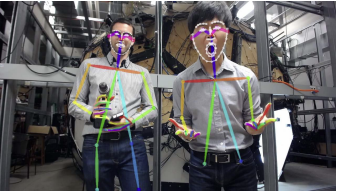
\includegraphics[height=1.5in]{figs/openpose.jpg} 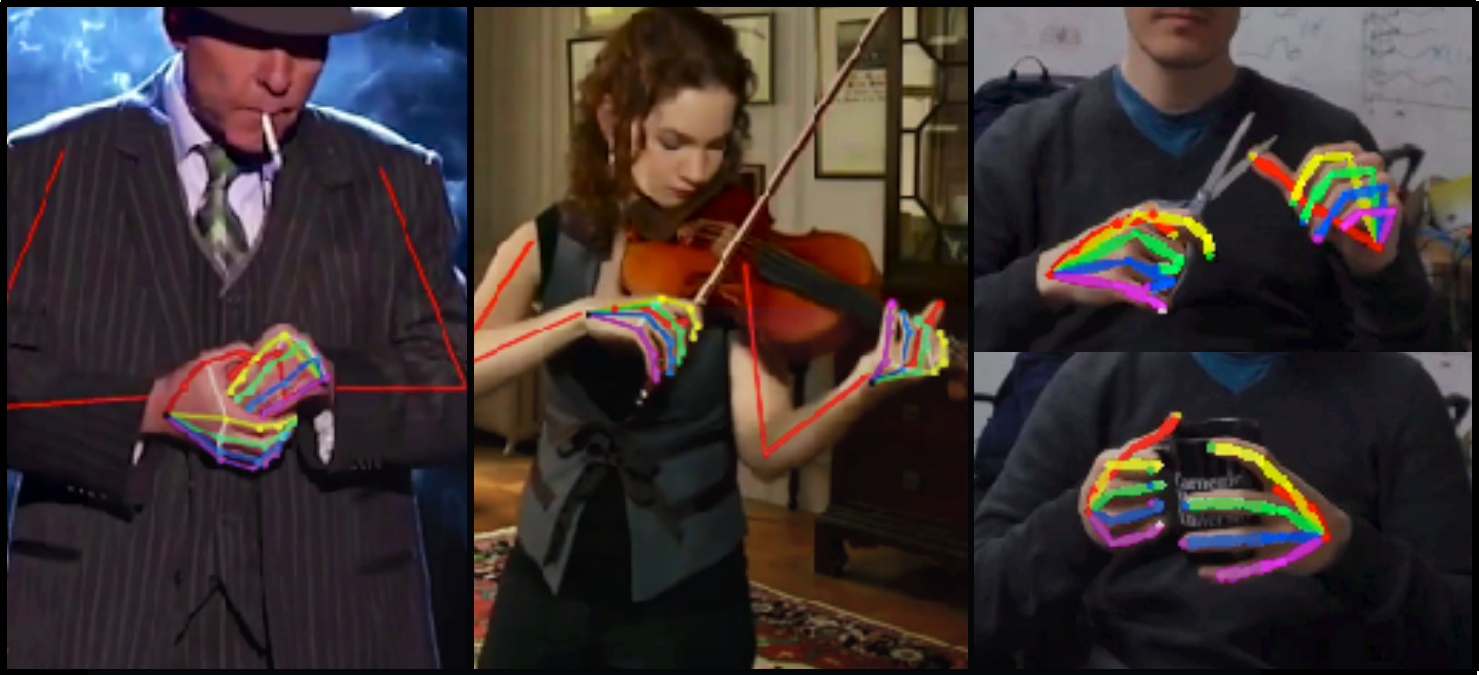
\includegraphics[height=1.5in]{figs/openpose2.jpg}}
    \caption[OpenPose Examples]{OpenPose Examples \cite{Cao2021,Simon2017}}
    \label{fig:openpose}
\end{figure}

\subsubsection{OpenPifPaf}

OpenPifPaf\cite{Kreiss2021,Kreiss2019}\footnote{OpenPifPaf documentation: \url{https://openpifpaf.github.io}} is an open-source project that aims to detect, associate, and track semantic keypoints. Detecting human joints is an example of its usage but it is also able to generalize this detection to other classes such as cars and animals. It can be installed as a Python package which can then be imported.

\begin{figure}[ht]
    \centering
    \adjincludegraphics[width=0.7\textwidth, trim={{0} {.05\height} {0} {.10\height}}, clip]{figs/openpifpaf.jpg}
    \caption[OpenPifPaf Example]{OpenPifPaf Example \cite{Kreiss2021}}
    \label{fig:openpifpaf}
\end{figure}

\subsubsection{MediaPipe}

% MediaPipe consists of a set of libraries and tools commonly used in \acs{ml} pipelines for advanced real-time vision-based applications \cite{Lugaresi2019}. The Hand Landmark Detection model \cite{Zhang2020} uses two sub-modules: a hand palm detection model and a hand landmark model. Each frame of an RGB input is fed into the palm detection model, which produces a bounding box based on the palm. The hand landmark model uses this bounding box and returns the keypoint localization of 21 landmarks, including the fingertips, the finger joints (knuckles), and the base of the palm. 

MediaPipe\footnote{MediaPipe documentation: \url{https://developers.google.com/mediapipe}} consists of a set of libraries and tools to apply \acs{ai} and \acs{ml} techniques in other applications, particularly in pipelines for advanced real-time vision-based applications \cite{Lugaresi2019}. Although it contains many features, in this work the focus is on the Hand and the Pose Landmark Detection Models.
The Hand Landmark Detection model \cite{Zhang2020} uses two sub-modules: a hand palm detection model and a hand landmark model. Each frame of an RGB input is fed into the palm detection model, which produces a bounding box based on the palm. The hand landmark model uses this bounding box and returns the keypoint localization of 21 landmarks, including the fingertips, the finger joints (knuckles), and the base of the palm (\autoref{fig:mediapipe_hand_landmarks}). The Pose Landmark Detection model also uses two sub-modules working in a similar way to return 33 landmarks over the entire body (\autoref{fig:mediapipe_pose_landmarks}). %Both of these models can be used to analyze both static images and continuous streams.


\if{0}

Just as the name suggests, the Hand Landmarker detects the landmarks of the hands (\autoref{fig:mediapipe_hand_landmarks}), and the Pose Landmarker detects the landmarks of the pose over the entire body (\autoref{fig:mediapipe_pose_landmarks}). These tasks use \acs{ml} models that can analyze both static images or a continuous stream and output the landmarks in the image and world coordinates as well as the handedness (left/right hand) of the detected hands in the case of the Hand Landmarker \cite{mediapipe_docs}.

The Hand Landmarker detects the landmarks of the hands in an image, as shown in Fig.~\ref{fig:mediapipe_hand_landmarks}. This task uses a machine learning (ML) model that can analyze both static data or a continuous stream and outputs the hand landmarks in image coordinates, hand landmarks in world coordinates, and handedness(left/right hand) of multiple detected hands.

The Pose Landmarker detects the landmarks of the pose over the entire body in an image, as shown in Fig.~\ref{fig:mediapipe_pose_landmarks}.  This task uses a machine learning (ML) model that can analyze both static data or a continuous stream and outputs the body pose landmarks in image coordinates and in 3-dimensional world coordinates.
\fi

\begin{figure}[ht]
    \centering
    \begin{subfigure}[b]{0.49\textwidth}
        \adjincludegraphics[width=\textwidth, trim={{.15\width} {0} {.05\width} {0}}, clip]{figs/hand_landmarker.jpg}
        \caption{}
        \label{fig:mediapipe_hand_landmarks}
    \end{subfigure} \
    \begin{subfigure}[b]{0.49\textwidth}
        \adjincludegraphics[width=\textwidth, trim={{0} {0} {.20\width} {0}}, clip]{figs/pose_landmarker.jpg}
        \caption{}
        \label{fig:mediapipe_pose_landmarks}
    \end{subfigure}
    \caption[Mediapipe landmarker models: Hand Landmarker and Pose Landmarker.]{Mediapipe landmarker models \cite{mediapipe_docs}: (a) Hand Landmarker and (b) Pose Landmarker.}
    \label{fig:mediapipe_landmarks}
\end{figure}

\subsection{\acfp{cnn}}

\acfp{cnn} are currently one of the most popular deep learning architectures and they are typically used to take advantage of the matrix structure of input data such as images and video where the input is too massive for other methods \cite{Sarker2021}. This architecture was originally introduced in a 1988 article \cite{Fukushima1988} and has since been further improved. According to \textcite{Alom2019}, the main building blocks are:
\begin{itemize}
    \item \textbf{Convolutional Layer}: in this layer, feature maps are extracted from receptive fields, which are parts of the input such as a region of pixels in an image or lower-level feature maps. This is done using a learnable kernel, consisting of a sliding window that goes through the entire input, computing the feature maps.

    \item \textbf{Sub-Sampling Layer}: this layer is responsible for downsampling the input feature maps effectively reducing the dimension of each feature map. It can also be named a pooling layer with the most common strategy being Max Pooling which simply returns the maximum value of the input.

    \item \textbf{Classification Layer}: this layer is composed of a variable number of fully connected layers that use the higher-level features computed in earlier layers to obtain the final scores of each class.
\end{itemize}

The global architecture is then described as the junction of two main parts: Feature Extractors and a Classifier (\autoref{fig:cnn_arch}). The first part is composed of one or more pairs of convolutional and pooling layers. The repetition of these layers makes it so the dimension of the features progressively decreases and higher-level features can eventually be derived from the the previous layers. Finally, the classifier is made up of fully-connected feed-forward layers and a final classifier layer and it is responsible for converting the higher-level feature maps into an array of scores for each class.

\begin{figure}[ht]
    \centering
    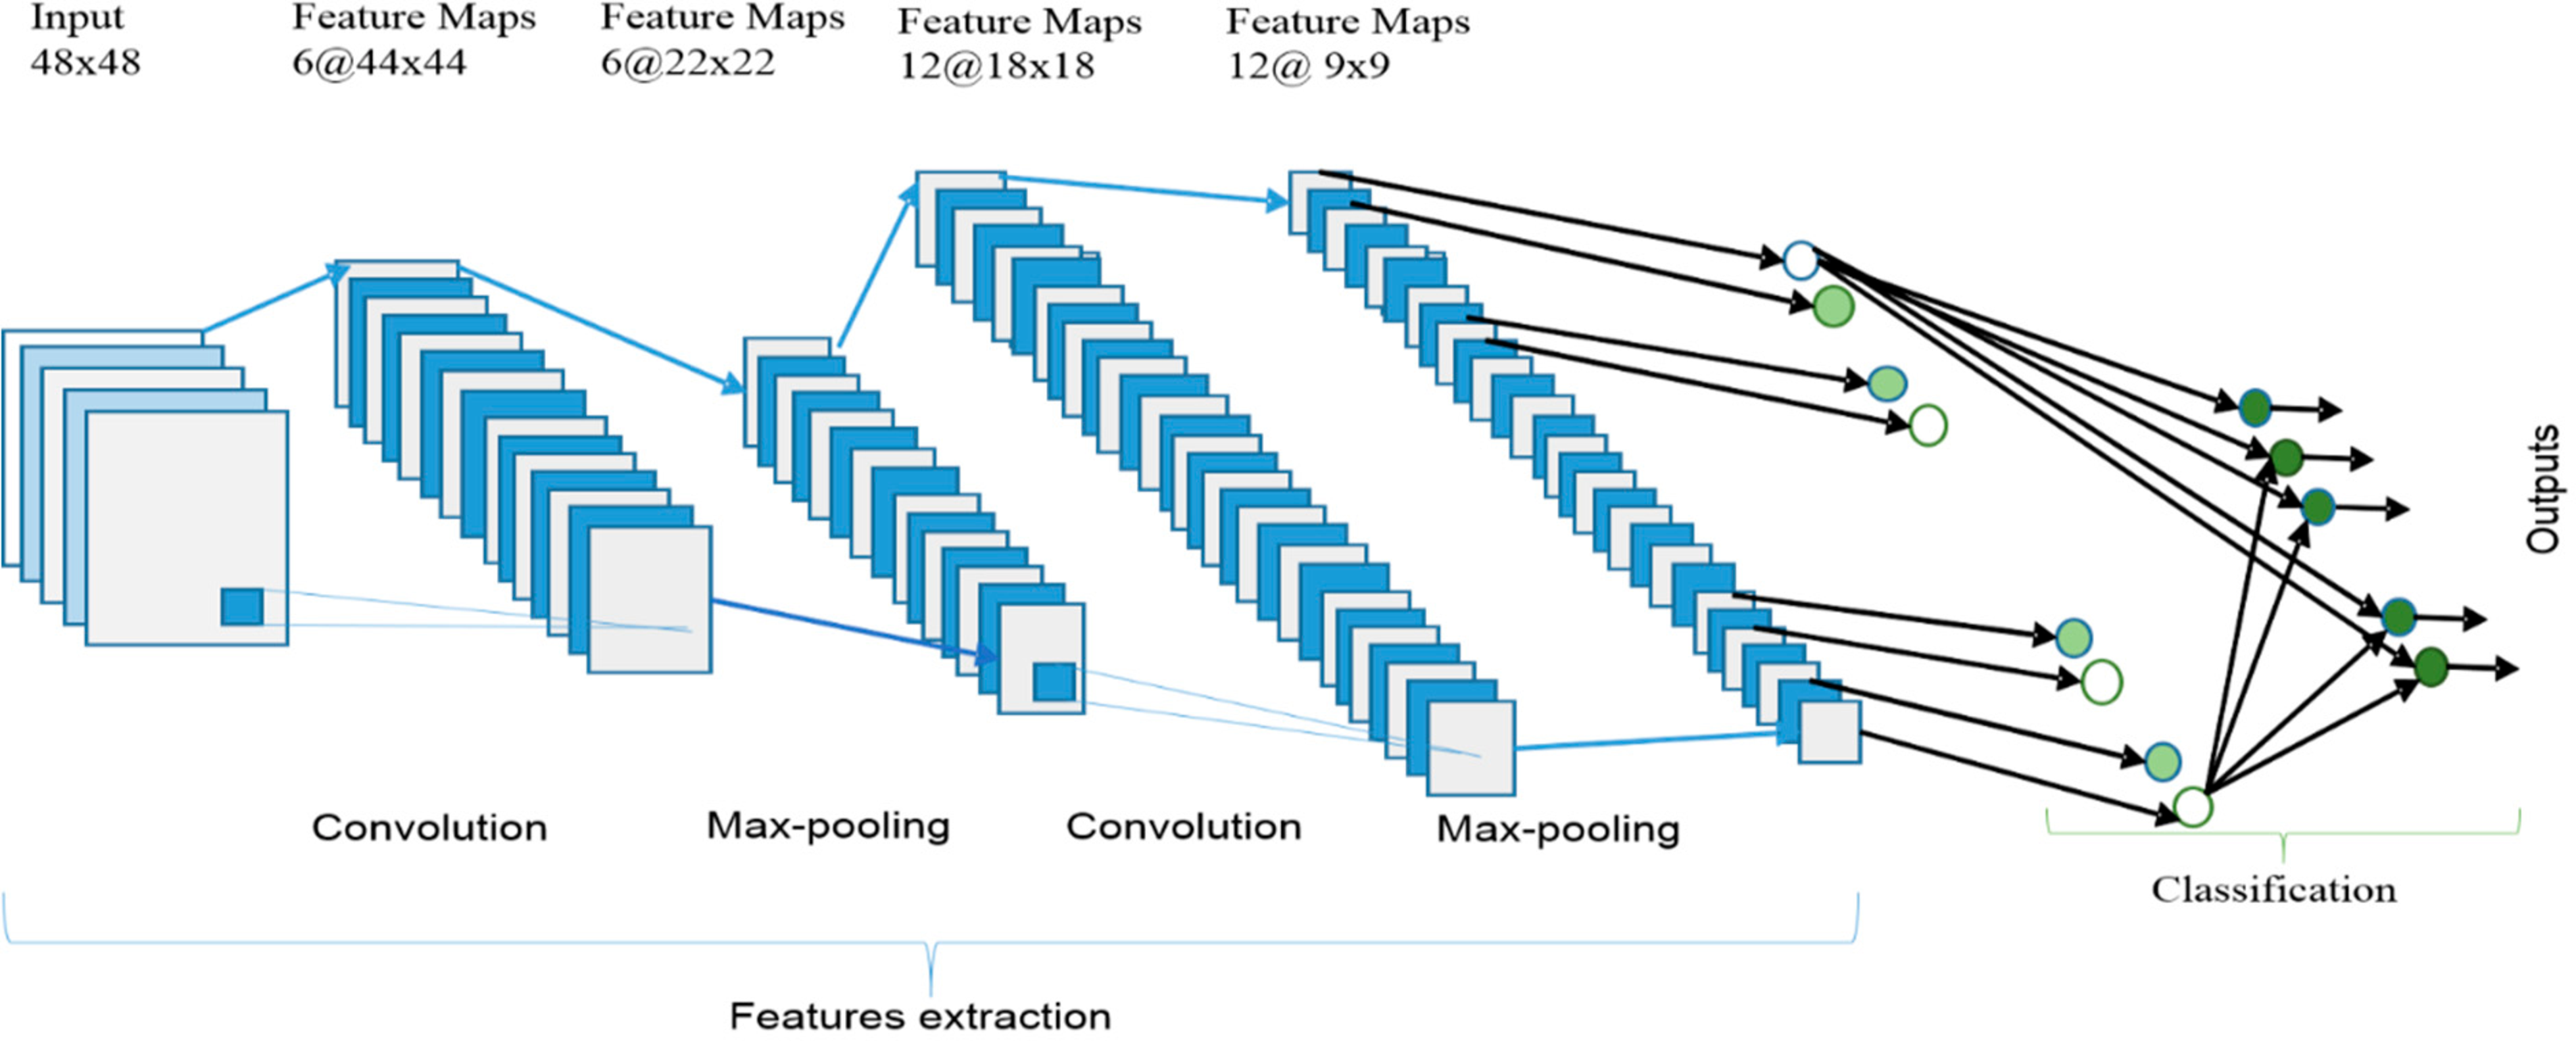
\includegraphics[width=1\textwidth]{figs/cnn_arch.pdf}
    \caption[\acs{cnn} Architecture]{\acs{cnn} Architecture \cite{Alom2019}}
    \label{fig:cnn_arch}
\end{figure}

\newpage

\subsection{Transformer Neural Networks}
\label{subsection:transformer_neural_networks}

Transformer Neural Networks consist of a new kind of neural network architecture that aims to solve tasks involving sequence data such as those in natural language processing. They were initially proposed in the "Attention Is All You Need" paper published by Google Research in 2017 \cite{Vaswani2017} and proceeded to surpass several established architectures in numerous tasks using attention mechanisms that identify complex relationships between elements in the input sequence. According to \textcite{Transformer_Oreilly}, the transformer's architectures are built upon 4 core concepts: % positional encoding, attention, self-attention, and multi-head (self-)attention.
\begin{itemize}
    \item \textbf{Positional Encoding} - \acs{rnn}s are able to work with sequences given that the tokens are processed sequentially. However, this approach comes with the disadvantage of the model having greater difficulty in analyzing long sequences, since important data might be forgotten. Transformers address this issue by using positional encoding, assigning a unique number to each token representing its position in the input sequence. This enables the transformer to learn the significance of each token's position.
    
    \item \textbf{Attention} - Attention is a concept that consists of measuring the relative importance of the input tokens to the output tokens. It was initially designed to facilitate language translation given that, when translating text from one language to the other, each word in the output can be influenced by multiple words from the input, and it became a key idea behind the transformer's architecture.

    \item \textbf{Self-attention} - Self-attention derives from attention but consists of measuring the relative importance of the input tokens to the other tokens of the input sequence instead of the output tokens. This concept allows the model to learn the relationships between tokens and their relevance in the input sequence even if they are far away.

    \item \textbf{Multi-head (self-)attention} - Multi-head (self-)attention refers to the fact that a transformer can have multiple attention heads. Each attention head performs a parallel process of (self-)attention allowing for multiple resulting weight matrices and, therefore, multiple definitions of relevance between the tokens.
\end{itemize}

The \autoref{fig:transformer_arch} shows the first published Transformer architecture. Initially, positional encodings are added to the input and output embeddings providing information about the relative positions. Then, in the encoder (left side of the figure), the input goes through a multi-head (self-)attention layer and a position-wise feedforward layer. In the decoder (right side of the figure), a different multi-head attention is applied on the output embeddings, and its output is used alongside the output of the encoder in another multi-head self-attention layer ending in a feedforward layer. Finally, the output of the last Transformer block is passed on to a dense layer converting it into a sequence of probabilities.

\begin{figure}[ht]
    \centerline{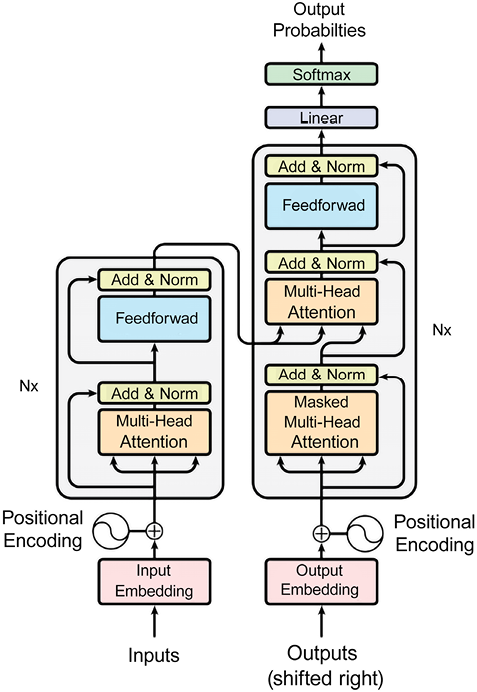
\includegraphics[width=0.6\textwidth]{figs/transformer.pdf}}
    \caption[Transformer Architecture]{Transformer Architecture \cite{Vaswani2017}}
    \label{fig:transformer_arch}
\end{figure}

\section{Integration of First Anticipation Experiments}
\label{section:first_experiments}

This section covers the integration of previously described tools and then the implementation of the first experiments to simulate anticipatory behavior in \acs{hrc}.

\subsection{Assembly Task: Build a Three-Color Flag}

To develop the necessary infrastructure, a concrete problem was needed. For this work, it was chosen to use sequences of big Lego blocks comparable to the stripes of a flag (\autoref{fig:flags_examples}). These blocks are initially placed behind the robot (\autoref{fig:table_workspace}), and the robot must fetch them and place them next to the user so that the user can build a flag. The blocks must be fetched in a certain order and there must be a way for the user to tell the robot that it is fetching the wrong block.

\begin{figure}[ht]
    \centering
    \begin{tikzpicture}[>=latex']

    \node (france_flag) {
\includegraphics[width=.2\textwidth]{figs/France.png}};
    \node[right =2cm of france_flag] (france_blocks) {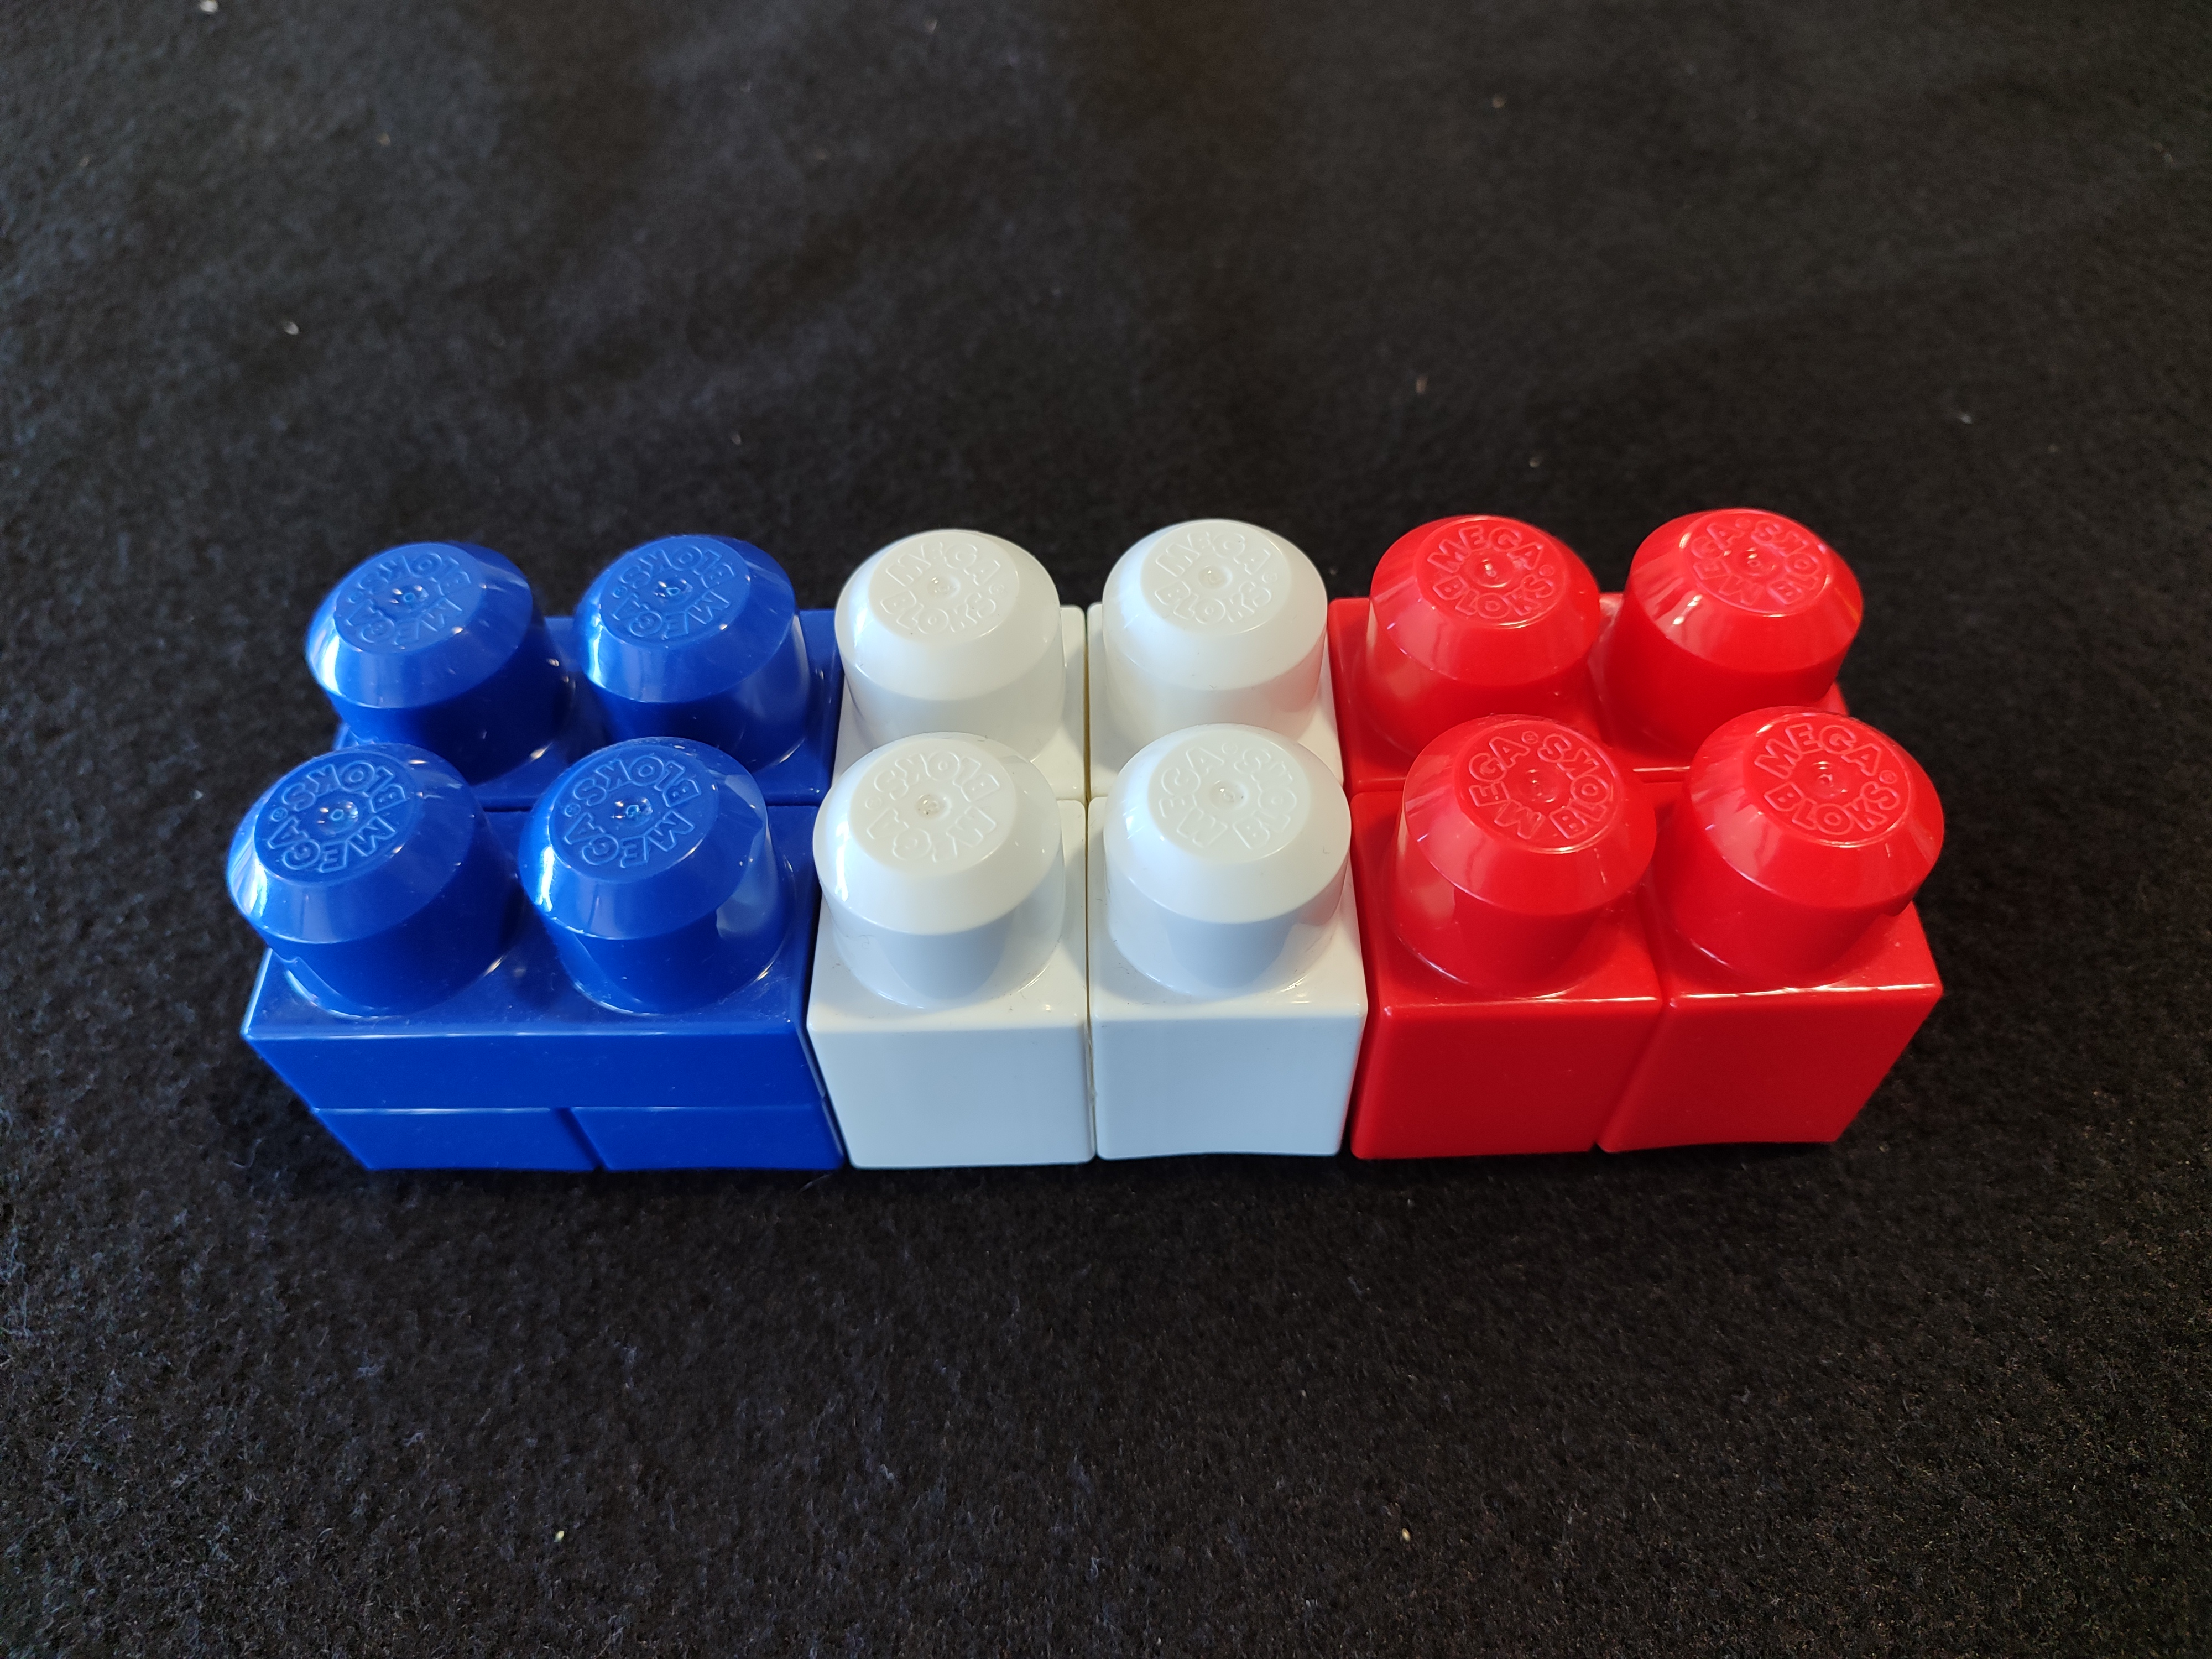
\includegraphics[width=.2\textwidth]{figs/flag1.jpg}};
    \node[below =0.3cm of france_flag] (portugal_flag) {
\includegraphics[width=.2\textwidth]{figs/Portugal.png}};
    \node[right =2cm of portugal_flag] (portugal_blocks) {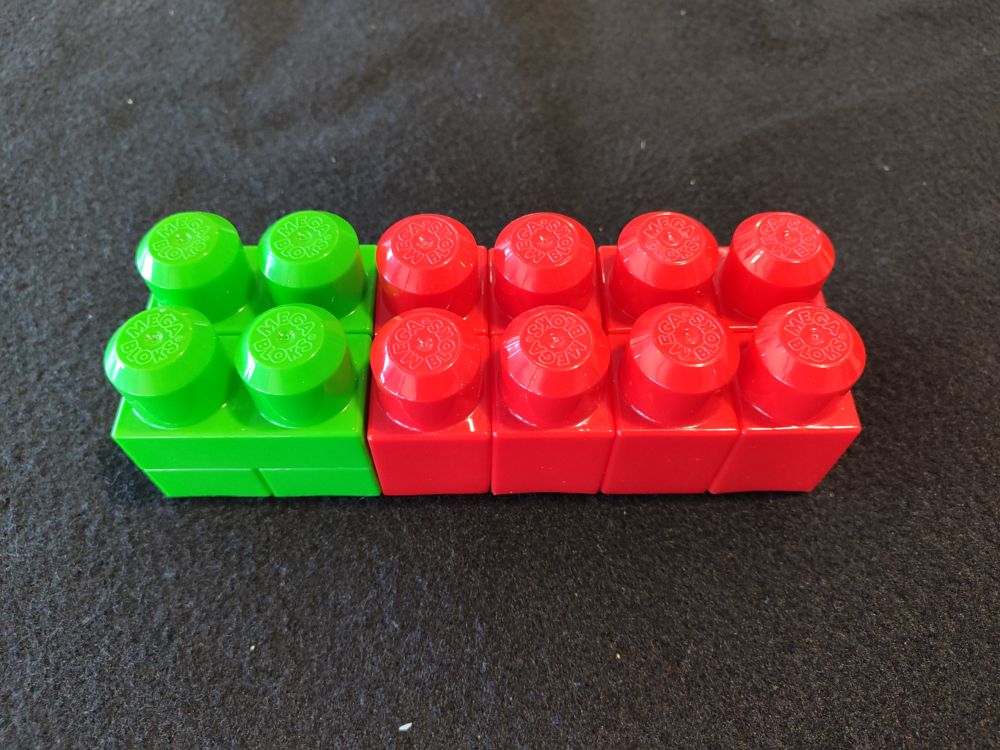
\includegraphics[width=.2\textwidth]{figs/flag2.jpg}};

    \path[draw, ->, text width=2cm, align=center]
        (france_flag) edge (france_blocks)
        (portugal_flag) edge (portugal_blocks)
    ;
    
\end{tikzpicture}
    \caption{Flag examples}
    \label{fig:flags_examples}
\end{figure}

\begin{figure}[ht]
    \centerline{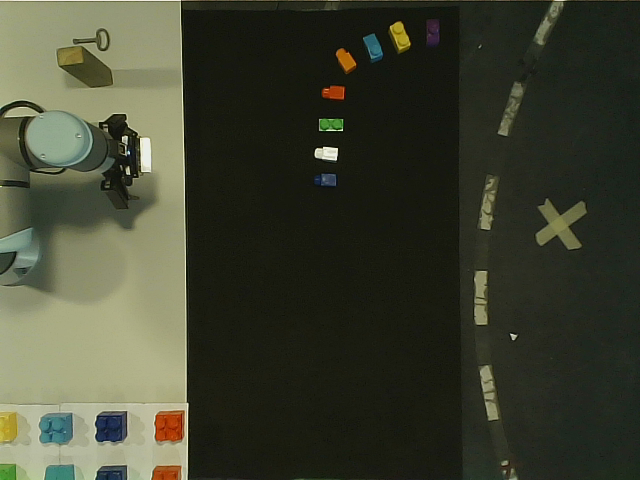
\includegraphics[width=0.7\textwidth]{figs/table_workspace.jpg}}
    \caption{Table workspace}
    \label{fig:table_workspace}
\end{figure}

Before the anticipation experiments, a base infrastructure was developed to build upon, integrating the perception system described in \autoref{subsection:perception_system} and the manipulator arm control system described in \autoref{subsection:manipulator_arm_control}. Connecting both of them is a decision-making node as shown in \autoref{fig:ros_architecture}. The logic in this node is implemented through a state machine with the behavior in each state corresponding to a method of a class, which facilitates the integration of additional logic by using subclasses of that class.

\begin{figure}[ht]
    \centering
    \begin{tikzpicture}[
        > = stealth, % arrow head style
        shorten > = 1pt, % don't touch arrow head to node
        auto,
        node distance = 4.5cm, % distance between nodes
        thick % line style
    ]
    
    \tikzstyle{every state}=[
        draw = black,
        thick,
        fill = white,
        minimum size = 4mm,
        text width = 2cm,
        align = center
    ]
    
    \node[state] (perception) {Perception System};
    \node[state] (decisionmaking) [right of=perception] {Decision Making};
    \node[state] (manipulator_arm_control) [right of=decisionmaking] {Manipulator Arm Control};

    \path[every edge,
    	->,
    	text width=1.8cm,
    	align=center
    	]
    (perception)       edge[bend left]  node {blocks position}        (decisionmaking)
    (perception)       edge[bend right]  node[below] {user position} (decisionmaking)
    (decisionmaking)   edge[bend left]  node {go to position/stop} (manipulator_arm_control)
    (manipulator_arm_control) edge[bend left] node {success/failure} (decisionmaking)
    ;

\end{tikzpicture}
    \caption{General \acs{ros} architecture with decision-making node}
    \label{fig:ros_architecture}
\end{figure}

The initial decision-making logic developed relied on interactions between the robot and the user. When the user puts his hand above a small block, if the robot is idle, then it proceeds to fetch a block of the same color. Additionally, when the user hovers his hand over the violet block while the robot is fetching a block, it means that the robot is fetching the wrong block, so it must stop and put the block back where it was before if it was already picked up. These interactions are also the fallback behavior if the methods in the following experiments fail to anticipate the block that the user desires.

\subsubsection{State Machine Logic}

As said before, the decision-making node contains an internal state machine. Although the logic of some states changes depending on the solution, all implementations follow the same general design represented in the state machine diagram shown in \autoref{fig:state_machine}.
\begin{figure}[ht]
    \centering
    \begin{tikzpicture}[
        > = stealth, % arrow head style
        shorten > = 1pt, % don't touch arrow head to node
        auto,
        node distance = 3.8cm, % distance between nodes
        thick % line style
    ]
    
    \tikzstyle{every state}=[
        draw = black,
        thick,
        fill = white,
        minimum size = 4mm,
        text width = 1.5cm,
        align = center
    ]
    
    \node[state] (idle) at (0,0) {idle};
    \node[state] (picking_up) [right of=idle] {picking up};
    \node[state] (moving_closer) [right of=picking_up] {moving closer};
    \node[state] (putting_down) [below of=picking_up] {putting down};
    \node[state] (stop_side_switch) [right of=moving_closer] {stop side switch};
    \node[state] (stop_wrong_guess) [above of=picking_up] {stop wrong guess};
    
    % \path[->] (idle) edge node[align=center] {received new\\sequence} (picking_up);
    % \path[->] (picking_up) edge node[align=center] {object\\picked up} (waiting);
    % \path[->] (waiting) edge node[align=center] {user\\finished} (moving_closer);
    % \path[->] (moving_closer) edge node[align=center] {robot in put\\down position} (putting_down);
    % \path[->] (putting_down) edge node[align=center] {object\\put down} (picking_up);
    % \path[->] (putting_down) edge[bend left] node[align=center] {sequence\\finished} (idle);
    % \path[->] (moving_closer) edge[bend left] node[align=center] {user changed\\side} (stop_side_switch);
    % \path[->] (stop_side_switch) edge[bend left] node[align=center] {robot\\stopped} (moving_closer);
    % \path[->] (picking_up) edge[bend right] node[align=center] {} (stop_wrong_guess);
    % \path[->] (waiting) edge node[align=center] {} (stop_wrong_guess);
    % \path[->] (moving_closer) edge[bend right] node[align=center] {wrong assembly\\sequence} (stop_wrong_guess);
    % \path[->] (stop_wrong_guess) edge[bend right] node[align=center] {reverted\\previous guess} (picking_up);

%Alternative lay-out for easier global configuration (vsantos)
\path[every edge,
	->,
	text width=1.8cm,
	align=center,
%	pos=0.4,
	]
(idle)             edge             node {knows which block is the next}   (picking_up)
(picking_up)       edge             node {object picked up}        (moving_closer)
(moving_closer)    edge[bend left]  node {robot in put down position} (putting_down)
(putting_down)     edge[bend left]  node {robot retreated}         (idle)
(moving_closer)    edge[bend left]  node {user changed side}       (stop_side_switch)
(stop_side_switch) edge[bend left]  node {robot stopped}           (moving_closer)
(picking_up)       edge             node[right] {wrong assembly sequence}                         (stop_wrong_guess)
(moving_closer)    edge[bend right]  node[above right] {wrong assembly sequence} (stop_wrong_guess)
(stop_wrong_guess) edge[bend right]  node[above left] {reverted previous guess} (idle)
; 
    
\end{tikzpicture}
    \caption{State machine diagram}
    \label{fig:state_machine}
\end{figure}
\begin{itemize}
    \item \textbf{idle}: state corresponding to when the robot does not know which is the next block. If the sequence has not started yet then it waits for the user to choose the first block and then the state changes to $picking$ $up$. If the sequence has already started then the database is fetched for the possible next blocks and then if at least one block is returned the state changes to $picking$ $up$ or if none is returned the system waits for the user to choose the next block.
    \item \textbf{picking up}: state corresponding to while the robot is picking up a certain block. After it picks it up the state changes to $moving$ $closer$ unless it was picking the wrong object in which case it changes to $stop$ $wrong$ $guess$.
    \item \textbf{moving closer}: state corresponding to the movement until the put-down position opposite to the user so that the robot does not constrain him. After the robot reaches the put-down position the state changes to $putting$ $down$. If the robot is holding the wrong object then the state changes to $stop$ $wrong$ $guess$ instead and if the user changes side the state changes to $stop$ $side$ $switch$.
    \item \textbf{putting down}: state corresponding to the movement necessary to put down the block in the table and the retreat of the robot outside the user's workspace. After that, the state changes to $idle$.
    \item \textbf{stop side switch}: State corresponding to the action of stopping the robot because the user changed sides. After the robot is stopped the state changes back to $moving$ $closer$.
    \item \textbf{stop wrong guess}: state corresponding to the action of stopping the robot because the user indicated that it was the wrong block. If the robot was already holding a block then that block is put back where it was while in this state. After the robot is stopped and it is not holding a block the state changes to $picking$ $up$ if there are still more possible blocks in the database. Otherwise, the state changes to $idle$ so that it waits for a user request.
\end{itemize}

\subsection{First Anticipation Experiments}
\label{subsection:first_anticipation_experiments}

This subsection describes the implementation and the workflow of the different experiments realized.

\subsubsection{Probability Based}

The first experiment consisted of having a database of probabilities that the robot would check to anticipate the block that the user would need next. In this experiment, when the decision-making node starts, it reads a configuration file with all the possible flags and then calculates and saves in a database the conditional probabilities of a certain color considering the previous ones.

When assembling a flag, the first block is still requested by the user but the following blocks are automatically given to the user according to the probabilities. However, if the robot chooses the wrong block the user can still communicate that fact by interacting with the small violet block and, if the robot exhausts all possibilities that it knows of, the user can request the following block using the interactions with the other small blocks.

\subsubsection{Rule Based}

The second experiment consisted of having a set of rules that the robot follows to anticipate the next block. These rules are read from a configuration file when the decision-making node starts and then managed by Experta\footnote{Experta documentation: \url{https://github.com/nilp0inter/experta}}. Experta is a Python library to create and deploy rule-based systems that make informed decisions using a knowledge base of rules. In this library, rules are defined as combinations of conditions and actions allowing for an intuitive syntax. Then, the engine uses these rules to make decisions using the declared information. For this experiment, some rules were defined about what should be the next block considering the blocks previously provided and the blocks rejected since the last accepted one.

Similarly to the previous experiment, the first block is requested by the user but for the following blocks, the robot checks if a rule is present for the current situation. If there is one, the robot follows that rule and provides a block and if there is not, it waits for the user to request the next block. The interactions for requesting and refusing a block are maintained.

\subsubsection{Rule Based + MediaPipe}

The third experiment is very similar to the previous one. The rule-based decision-making is maintained with the same rules but the first block is no longer requested by the user. Instead, the user picks up the first block and the second camera which is facing the user detects the color of the object. To do this, the pose model from MediaPipe is used to detect the position of the hands which is then used to crop the received image to a region of interest. The resulting image is segmented similarly to the images of the other camera and if a color is detected, then that color is considered the color of the first block.

\section{Final Remarks}
\label{section:materials_methods_final_remarks}

This chapter reviewed the necessary components to create a \acf{hrc} system starting with the provided collaboration cell and how the different components are set up and are able to establish communication using \acs{ros}. Then, the different tools that constitute this research are further described which were the keypoint detection frameworks, in particular MediaPipe, the \acfp{cnn}, and the Transformer Neural Networks. Finally, all components are connected with a decision-making node which handles which actions the robot should take. The first implementation included a database of probabilities that guided which action the robot should take but this solution proved to have reduced flexibility. Then, the second implementation used Experta to set up a list of rules to decide the action the robot should take next with a configuration file, a characteristic that made the robot's behavior more flexible since the rules could be easily changed. Finally, the last implementation integrated MediaPipe not only to reduce the direct communication between the robot and the user but also in preparation for its use in the next chapter.